% Figure 1: overview of the evaluation framework. Drawn at the RSOS text width (135 mm).
\documentclass[border=1mm]{standalone}
\usepackage[T1]{fontenc}
\usepackage[scaled=0.92]{helvet}
\renewcommand\familydefault{\sfdefault}
\usepackage{amssymb}
\usepackage{tikz}
\usetikzlibrary{arrows.meta,calc,shapes.geometric}
% ---- shared style (all four methodology figures) ----
\definecolor{mA}{HTML}{1B7F79}\definecolor{mAl}{HTML}{E4F2F0}
\definecolor{mB}{HTML}{2F5F98}\definecolor{mBl}{HTML}{E7EEF7}
\definecolor{mC}{HTML}{B85A16}\definecolor{mCl}{HTML}{FBEEDF}
\definecolor{ink}{HTML}{262626}\definecolor{mute}{HTML}{666666}
\definecolor{rule}{HTML}{BDBDBD}\definecolor{grey}{HTML}{8C8C8C}\definecolor{greyl}{HTML}{EFEFEF}
\newcommand\fs{\fontsize{7}{8.4}\selectfont}
\newcommand\fss{\fontsize{6.3}{7.5}\selectfont}
\newcommand\fsh{\fontsize{7.6}{9}\selectfont\bfseries}
\hyphenpenalty=10000 \exhyphenpenalty=10000
\tikzset{
  >={Stealth[length=2mm,width=1.6mm]},
  flow/.style={->,line width=0.8pt,draw=ink!75},
  netnode/.style={circle,fill=#1,inner sep=0pt,minimum size=1.3mm},
}
% database icon: \dbicon{colour}{(x,y)}{scale}
\newcommand\dbicon[3]{\begin{scope}[shift={#2},scale=#3]
  \filldraw[fill=#1!16,draw=#1,line width=0.5pt] (-2,2) -- (-2,-2) arc[start angle=180,end angle=360,x radius=2,y radius=0.7] -- (2,2);
  \draw[#1,line width=0.4pt] (-2,0) arc[start angle=180,end angle=360,x radius=2,y radius=0.7];
  \filldraw[fill=#1!40,draw=#1,line width=0.5pt] (0,2) ellipse[x radius=2,y radius=0.7];
\end{scope}}
% network icon: \neticon{colour}{(x,y)}{scale}
\newcommand\neticon[3]{\begin{scope}[shift={#2},scale=#3]
  \draw[#1,line width=0.45pt] (-2,-1.4)--(0,1.6)--(2,-1.4)--cycle (0,1.6)--(0,-0.2)--(-2,-1.4) (0,-0.2)--(2,-1.4);
  \foreach \p in {(-2,-1.4),(0,1.6),(2,-1.4),(0,-0.2)} \node[netnode=#1] at \p {};
\end{scope}}
% detail card: \dcard{colour}{x-left}{y-top}{width}{height}{title}
\newcommand\dcard[6]{%
  \fill[#1l,rounded corners=1.4mm] (#2,#3) rectangle ++(#4,-#5);
  \draw[#1,line width=0.6pt,rounded corners=1.4mm] (#2,#3) rectangle ++(#4,-#5);
  \fill[#1,rounded corners=1.4mm] (#2,#3) rectangle ++(#4,-5.2);
  \fill[#1] ($(#2,#3)+(0,-5.2)$) rectangle ++(#4,1.6);
  \node[anchor=west,text=white,font=\fs\bfseries] at ($(#2,#3)+(1.4,-2.6)$) {#6};}
% plain step box: \sbox{colour}{x0}{y0}{x1}{y1}{text}
\newcommand\stepbox[6]{%
  \fill[white,rounded corners=1.2mm] (#2,#3) rectangle (#4,#5);
  \draw[#1,line width=0.6pt,rounded corners=1.2mm] (#2,#3) rectangle (#4,#5);
  \node[font=\fss,text width=(#4-#2-2)*1mm,align=center] at ({(#2+#4)/2},{(#3+#5)/2}) {#6};}
% leakage marker (unlabelled held-out expression used)
\newcommand\leak[1]{\node[diamond,fill=mC,inner sep=0pt,minimum size=2.6mm] at #1 {};}
% module card: #1 colour, #2 x-left, #3 number, #4 title, #5 body, #6 key numbers (width 40 mm)
\newcommand\card[6]{%
  \fill[#1l,rounded corners=1.6mm] (#2,33) rectangle ++(40,26);
  \draw[#1,line width=0.7pt,rounded corners=1.6mm] (#2,33) rectangle ++(40,26);
  \fill[#1,rounded corners=1.6mm] (#2,59) rectangle ++(40,-6.5);
  \fill[#1] (#2,52.5) rectangle ++(40,2);
  \node[circle,fill=white,text=#1,inner sep=0pt,minimum size=4.4mm,font=\fss\bfseries] at (#2+3.4,55.75) {#3};
  \node[anchor=west,text=white,font=\fsh,text width=32mm,align=left] at (#2+6.4,55.75) {#4};
  \node[anchor=north west,text=ink,font=\fs,text width=36.5mm,align=left] at (#2+1.6,51.6) {#5};
  \node[anchor=south west,text=#1,font=\fs\bfseries,text width=36.5mm,align=left] at (#2+1.6,34) {#6};
}
\newcommand\tile[4]{% #1 x, #2 id, #3 name (two lines), #4 question
  \fill[white,rounded corners=1.2mm] (#1,4.2) rectangle ++(20.4,19.8);
  \draw[mC!70,line width=0.5pt,rounded corners=1.2mm] (#1,4.2) rectangle ++(20.4,19.8);
  \fill[mC,rounded corners=1.2mm] (#1,24) rectangle ++(20.4,-7.6);
  \fill[mC] (#1,16.4) rectangle ++(20.4,1.5);
  \node[circle,fill=white,text=mC,inner sep=0pt,minimum size=4.2mm,font=\fss\bfseries] at (#1+2.9,20.2) {#2};
  \node[anchor=west,text=white,font=\fss\bfseries,text width=14.6mm,align=left] at (#1+5.4,20.2) {#3};
  \node[anchor=north,font=\fss,text width=19mm,align=center] at (#1+10.2,15.6) {#4};}
\begin{document}
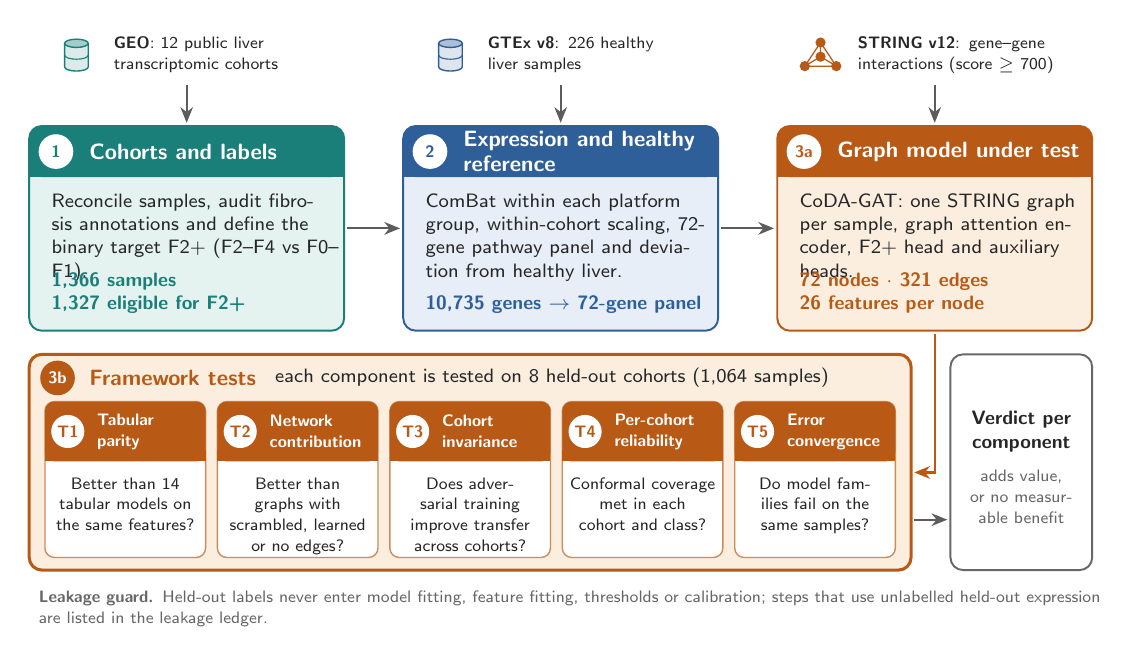
\begin{tikzpicture}[x=1mm,y=1mm,font=\fs,text=ink]
% ---------------- inputs ----------------
\dbicon{mA}{(6,68)}{0.75}
\node[anchor=west,font=\fss,text width=30mm,align=left] at (9.5,68) {\textbf{GEO}: 12 public liver\\transcriptomic cohorts};
\dbicon{mB}{(53.5,68)}{0.75}
\node[anchor=west,font=\fss,text width=30mm,align=left] at (57,68) {\textbf{GTEx v8}: 226 healthy\\liver samples};
\neticon{mC}{(100.5,68)}{1}
\node[anchor=west,font=\fss,text width=31mm,align=left] at (104,68) {\textbf{STRING v12}: gene--gene\\interactions (score $\geq$ 700)};
\foreach \x in {20,67.5,115} \draw[flow,line width=0.6pt] (\x,64.2)--(\x,59.4);
% ---------------- modules ----------------
\card{mA}{0}{1}{Cohorts and labels}
  {Reconcile samples, audit fibrosis annotations and define the binary target F2+ (F2--F4 vs F0--F1).}
  {1,366 samples\\1,327 eligible for F2+}
\card{mB}{47.5}{2}{Expression and healthy reference}
  {ComBat within each platform group, within-cohort scaling, 72-gene pathway panel and deviation from healthy liver.}
  {10,735 genes $\rightarrow$ 72-gene panel}
\card{mC}{95}{3a}{Graph model under test}
  {CoDA-GAT: one STRING graph per sample, graph attention encoder, F2+ head and auxiliary heads.}
  {72 nodes $\cdot$ 321 edges\\26 features per node}
\draw[flow] (40.4,46)--(47.1,46);
\draw[flow] (87.9,46)--(94.6,46);
% ---------------- framework band (module 3b, emphasised) ----------------
\fill[mCl,rounded corners=1.6mm] (0,2.6) rectangle (112,30);
\draw[mC,line width=1.1pt,rounded corners=1.6mm] (0,2.6) rectangle (112,30);
\node[circle,fill=mC,text=white,inner sep=0pt,minimum size=4.4mm,font=\fss\bfseries] at (3.6,27) {3b};
\node[anchor=west,font=\fsh,text=mC] at (6.4,27) {Framework tests};
\node[anchor=west,font=\fs,text=ink] at (30,27) {each component is tested on 8 held-out cohorts (1,064 samples)};
\draw[flow,draw=mC] (115,32.6) |- (112.4,15);
\tile{2}{T1}{Tabular\\parity}{Better than 14 tabular models on the same features?}
\tile{23.9}{T2}{Network\\contribution}{Better than graphs with scrambled, learned or no edges?}
\tile{45.8}{T3}{Cohort\\invariance}{Does adversarial training improve transfer across cohorts?}
\tile{67.7}{T4}{Per-cohort\\reliability}{Conformal coverage met in each cohort and class?}
\tile{89.6}{T5}{Error\\convergence}{Do model families fail on the same samples?}
% ---------------- output ----------------
\fill[white,rounded corners=1.6mm] (117,2.6) rectangle (135,30);
\draw[ink!70,line width=0.7pt,rounded corners=1.6mm] (117,2.6) rectangle (135,30);
\draw[flow] (112.4,9)--(116.6,9);
\node[anchor=north,font=\fs\bfseries,text width=17mm,align=center] at (126,24) {Verdict per component};
\node[anchor=north,font=\fss,text width=17mm,align=center,text=mute] at (126,16.5) {adds value, or no measurable benefit};
% ---------------- leakage guard ----------------
\node[anchor=north west,font=\fss,text=mute,text width=135mm,align=left] at (0,1.2)
  {\textbf{Leakage guard.} Held-out labels never enter model fitting, feature fitting, thresholds or calibration; steps that use unlabelled held-out expression are listed in the leakage ledger.};
\end{tikzpicture}
\end{document}
